\section{模拟信号与数字信号}

\begin{frame}
    \frametitle{模拟信号}
        \begin{minipage}{0.48\linewidth}
            \highlight{模拟信号}是指用连续变化的物理量所表达的信息，如温度、湿度、压力、长度、电流、电压等等。实际生产生活中的各种物理量都是模拟信号。

    我们通常又把模拟信号称为\highlight{连续信号}，其信号的幅度，或频率，或相位随时间作连续变化，或在一段连续的时间间隔内，其代表信息的特征量可以在任意瞬间呈现为任意数值的信号。

    % 模拟信号传输过程中，先把信息信号转换成几乎“一模一样”的波动电信号(因此叫“模拟”)，再通过有线或无线的方式传输出去，电信号被接收下来后，通过接收设备还原成信息信号。
        \end{minipage}\hfill        
        \begin{minipage}{0.48\linewidth}
            \begin{center}
                \begin{tikzpicture}[scale=0.5]
                    \draw [->] (0,0) -- (13,0);
                    \draw [->] (0,0) -- (0,5);
                    \node at (0,0) [below] {0};
                    \node at (13,0) [below] {$t$};
                    \node at (0,5) [left] {$u$};
                    \draw[domain=0:12.56,smooth] plot(\x,{2*sin(\x r)});
                \end{tikzpicture}
            \end{center}
        \end{minipage}
    

\end{frame}

\begin{frame}
    \frametitle{模拟信号的优点}
    \begin{itemize}
      \item \cbf{精确的分辨率}
      
      在理想情况下，它具有无穷大的分辨率。与数字信号相比，模拟信号的信息密度更高。由于不存在量化误差，它可以对自然界物理量的真实值进行尽可能逼近的描述。

      \item \cbf{处理简单}
      
      当达到相同的效果，模拟信号处理比数字信号处理更简单。模拟信号的处理可以直接通过模拟电路组件（例如运算放大器等）实现，而数字信号处理往往涉及复杂的算法，甚至需要专门的数字信号处理器。
    \end{itemize}
\end{frame}

\begin{frame}
    \frametitle{模拟信号的缺点}
    \begin{minipage}{0.58\linewidth}
        近百年以来，无论是有线相连的电话，还是无线发送的广播电视，很长的时间内都是用模拟信号来传递信号的。照说模拟信号同原始信号在波形上几乎“一模一样”，似乎应该达到很好的传播效果，然而事实恰恰相反，这是因为信号在传输过程中要经过许多的处理和转送，产生各种干扰。

    模拟信号的主要缺点是它总是受到杂讯的影响。信号被多次复制，或进行长距离传输之后，这些随机噪声的影响可能会变得十分显著。
    \end{minipage}\hfill
    \begin{minipage}{0.38\linewidth}
        \begin{figure}[htpb]
            \centering
            
\includegraphics[width=\linewidth]{images/我听不见}
        \end{figure}
    \end{minipage}
\end{frame}

\begin{frame}
    \frametitle{数字信号}
        \begin{minipage}{0.48\linewidth}
            \highlight{数字信号}是指用一组特殊的状态来描述信号，典型的就是当前用最为常见的二进制数字来表示的信号。

    数字信号与模拟信号不同，它的自变量是离散的、因变量也是离散的，这种信号的自变量用整数表示，因变量用有限数字中的一个数字来表示。

    在实际的数字信号传输中，通常是将一定范围的信息变化归类为状态0或状态1， 这种状态的设置大大提高了数字信号的抗噪声能力。
        \end{minipage}\hfill
        \begin{minipage}{0.5\linewidth}
            \begin{center}
                \begin{tikzpicture}[scale=0.5]
                    \draw [->] (0,0) -- (13,0);
                    \draw [->] (0,0) -- (0,5);
                    \node at (0,0) [below] {0};
                    \node at (13,0) [below] {$t$};
                    \node at (0,5) [left] {$u$};
                    \draw (2,0) rectangle (4,4);
                    \draw[shift = {(4,0)}] (2,0) rectangle (4,4);
                \end{tikzpicture}
            \end{center}
        \end{minipage} 
\end{frame}

\begin{frame}
    \frametitle{数字信号的优点}
        \begin{minipage}{0.5\linewidth}
            \begin{itemize}
                \item 抗干扰能力强，无噪声积累
                \item 便于加密处理
                \item 便于储存、处理和交换
                \item 设备便于集成化、微型化
                \item 便于构建综合数字通信网
              \end{itemize}
        \end{minipage}\hfill
        \begin{minipage}{0.48\linewidth}
            \begin{figure}[htpb]
                \centering
                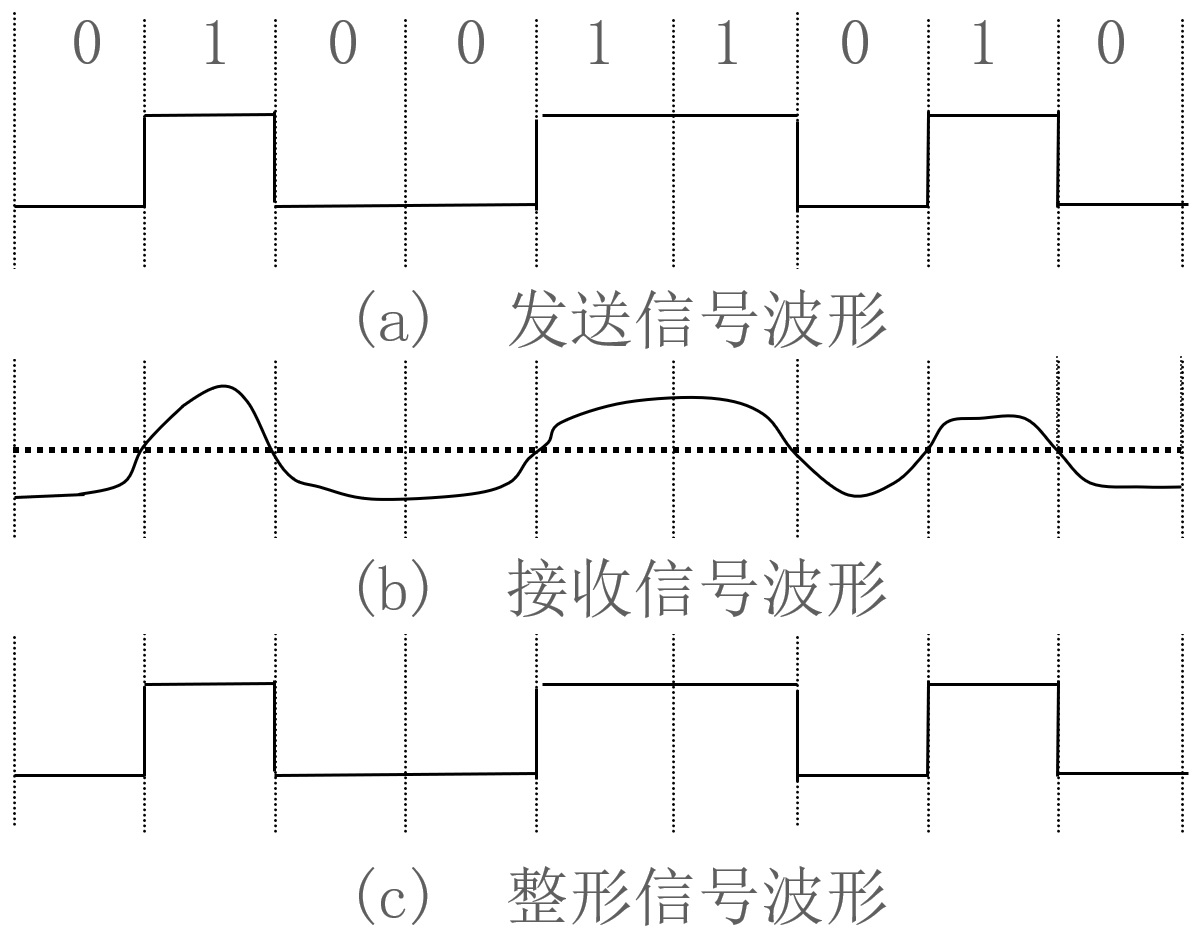
\includegraphics[width=\linewidth]{images/数字信号整形}
            \end{figure}
        \end{minipage}
\end{frame}


\begin{frame}
    \frametitle{数字信号的缺点}
    \begin{itemize}
      \item 增加了系统的复杂性
      \item 占用频带较宽，信号频率高
      \item 系统的功率消耗比较大
      \item 进行模/数转换时会带来量化误差
    \end{itemize}
\end{frame}

\begin{frame}
    \frametitle{模拟信号转换为数字信号}
        \begin{minipage}{0.48\linewidth}
            \begin{enumerate}
                \item \cbf{采样}
                
                把模拟信号由时间上连续变为时间上离散的。
                \item \cbf{量化}
                
                采样完了的信号时间上是离散的，间隔了若干周期才变化。但是因变量的取值仍然是随意的。那么在接下来的过程中，通过把这些因变量映射到固定的数值上去。
                \item \cbf{编码}
                
                以特定的二进制数值系统表征。
              \end{enumerate}
        \end{minipage}\hfill
        \begin{minipage}{0.5\linewidth}
            \begin{center}

                \only<1>{
                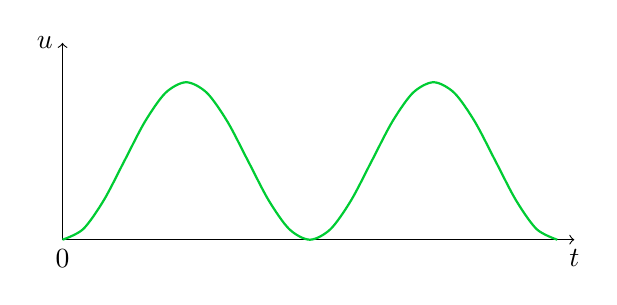
\begin{tikzpicture}[scale=0.5]
                    \draw [->] (0,0) -- (13,0);
                    \draw [->] (0,0) -- (0,5);
                    \node at (0,0) [below] {0};
                    \node at (13,0) [below] {$t$};
                    \node at (0,5) [left] {$u$};
                    \draw[domain=0:4*pi,smooth,thick,blue!20!green] plot(\x ,{2*sin((\x-pi/2) r)+2});
                \end{tikzpicture}
                }

                \only<2>{
                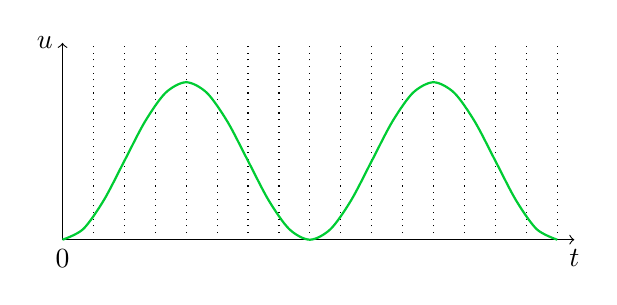
\begin{tikzpicture}[scale=0.5]
                    \draw [->] (0,0) -- (13,0);
                    \draw [->] (0,0) -- (0,5);
                    \foreach \x in {pi/4,2*pi/4,3*pi/4,4*pi/4,5*pi/4,6*pi/4,7*pi/4,8*pi/4,9*pi/4,10*pi/4,11*pi/4,12*pi/4,13*pi/4,14*pi/4,15*pi/4,16*pi/4}
                    \draw [dotted] (\x,0) -- (\x,5);
                    \node at (0,0) [below] {0};
                    \node at (13,0) [below] {$t$};
                    \node at (0,5) [left] {$u$};
                    \draw[domain=0:4*pi,smooth,thick,blue!20!green] plot(\x ,{2*sin((\x-pi/2) r)+2});
                \end{tikzpicture}
                }

                \only<3>{
                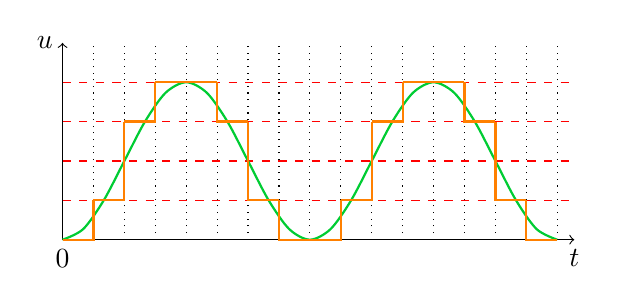
\begin{tikzpicture}[scale=0.5]
                    \draw [->] (0,0) -- (13,0);
                    \draw [->] (0,0) -- (0,5);
                    \foreach \x in {pi/4,2*pi/4,3*pi/4,4*pi/4,5*pi/4,6*pi/4,7*pi/4,8*pi/4,9*pi/4,10*pi/4,11*pi/4,12*pi/4,13*pi/4,14*pi/4,15*pi/4,16*pi/4}
                    \draw [dotted] (\x,0) -- (\x,5);
                    \foreach \x in {1,2,3,4}
                    \draw [red,dashed] (0,\x) -- (13,\x);
                    \node at (0,0) [below] {0};
                    \node at (13,0) [below] {$t$};
                    \node at (0,5) [left] {$u$};
                    \draw[domain=0:4*pi,smooth,thick,blue!20!green] plot(\x ,{2*sin((\x-pi/2) r)+2});
                    \draw[thick,orange] (0,0) -| (pi/4,1);
                    \draw[thick,orange] (pi/4,1) -| (pi/2,3);
                    \draw[thick,orange] (pi/2,3) -| (3*pi/4,4);
                    \draw[thick,orange] (3*pi/4,4) -| (5*pi/4,4);
                    \draw[thick,orange] (5*pi/4,4) |- (6*pi/4,3);
                    \draw[thick,orange] (6*pi/4,3) |- (7*pi/4,1);
                    \draw[thick,orange] (7*pi/4,1) |- (2*pi,0);
                    \draw[thick,orange,shift={(2*pi,0)}] (0,0) -| (pi/4,1);
                    \draw[thick,orange,shift={(2*pi,0)}] (pi/4,1) -| (pi/2,3);
                    \draw[thick,orange,shift={(2*pi,0)}] (pi/2,3) -| (3*pi/4,4);
                    \draw[thick,orange,shift={(2*pi,0)}] (3*pi/4,4) -| (5*pi/4,4);
                    \draw[thick,orange,shift={(2*pi,0)}] (5*pi/4,4) |- (6*pi/4,3);
                    \draw[thick,orange,shift={(2*pi,0)}] (6*pi/4,3) |- (7*pi/4,1);
                    \draw[thick,orange,shift={(2*pi,0)}] (7*pi/4,1) |- (2*pi,0);
                \end{tikzpicture}
                }
            \end{center}
        \end{minipage}
\end{frame}


\begin{frame}[t]
    \frametitle{}
    \begin{question}
        能不能不断提高采样率和量化位数，使数字音频的质量达到模拟声音的质量？
        \tcblower
        \pause
        从原理上讲通过不断提高采样率和量化位数来提高数字音频的质量是可行的。

        但是实际生活中：
        \begin{enumerate}
          \item 这样会大大增加保存信息的数据量以及信息处理量
          \item 我们的耳朵分辨能力也是有限的，过高的采样率和量化位数会造成浪费
        \end{enumerate}
        
    \end{question}
\end{frame}